\chapter{Højtaler \& Kabinet}

\section{Teori}
Højtaleren der benyttes til projektet er en 6.5" mellemtone elektrodynamisk højtaler af mærket FW168\cite{FW168} fra firmaet Fountek \cite{Fountek}. 

På figur \ref{fig:kompletmodel} ses den komplette model for højtalerens elektriske, mekaniske og akustiske system.\citep{Elektroakustik} Komponentværdierne og forklaringen af disse, kan ses i tabel YY.\fixme{Opret tabel med Thiele-Small værdier LS}

\begin{figure}[H]
	\centering
	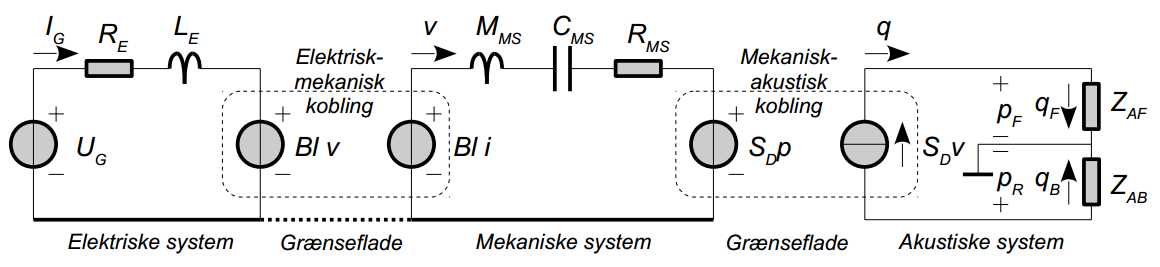
\includegraphics[width=\textwidth]{Pics/kompletmodel.PNG}
	\label{fig:kompletmodel}
	\caption{Komplet model fro højtalerens elektrisk, mekaniske- og akustiske system. } 
\end{figure}

Omregner man modellen til en komplet elektrisk model, kan man udregne den elektrsiek impedans $Z_E$ for modellen. Denne impedans har et toppunkt ved højtalerens resonansfrekvens, og en minimumsværdi ved svingspolens $R_E$-værdi.

Med værdierne fra tabel YY udregnes den elektriske impedans for højtaleren i ligning \ref{eq:eq1}

\begin{equation}\label{eq:eq1}
Z_E(s)=R_E+sL_E+\frac{Bl^2}{\omega_s M_{MS}} \frac{ \omega_s s}{ s^2 + \frac{1}{Q_{MS}} \omega_s s + \omega_s^2} \end{equation} \begin{equation} \ \qquad  = 
7.2\Omega + s \cdot 1mH + \frac{(8.2 Tm)^2}{287.8Hz \cdot 14.7gm} \frac{ 287.8Hz \cdot s}{ s^2 + \frac{1}{3.246} 287.8Hz \cdot s + (287.8Hz)^2}  \end{equation}

Impedansen vil være størst ved højtalerensresonansfrekvens $f_s$, som beregnes i ligning \ref{eq:fs}

\begin{equation}\label{eq:fs}
f_s=\frac{1}{2 \pi \sqrt{M_{MS} C_{MS}}}=45.813Hz
\end{equation}

På figur \ref{fig:ZE_graf} \fixme{Find ud af at lave det i matlab!!!! LS} ses plottet af ligning \ref{eq:eq1} med værdierne for højtaleren. Kurveforløbet stemmer overens med det beregnede toppunkt $f_s$ og minimumsværdien $R_E$. Kurveforløbet stemmer ligeledes overens med det opgivne i databladet \cite{FW168}.

\begin{figure}[H]
	\centering
	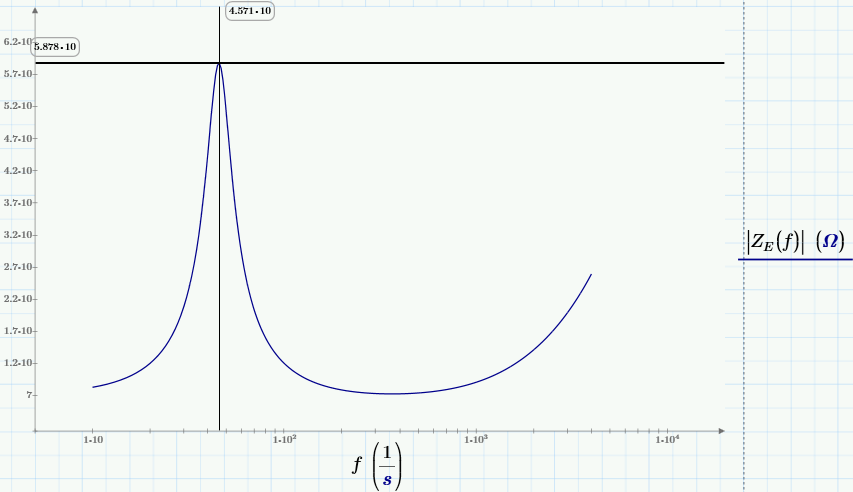
\includegraphics[width=\textwidth]{Pics/ZE_graf.PNG}
	\label{fig:ZE_graf}
	\caption{Den elektriske impedans $Z_E$ som funktion af frekvensen} 
\end{figure}

\section{Simulering}

\newpage
\section{Realisering}
Højtalerens og kabinettets frekvenskarakteristik blev målt ved hjælp af en såkaldt CLIO Pocket. Der kan læses mere omkring dette værktøj og målemetoden i kapitel \ref{ch:measurements}; men det centrale er, at der måles på et frekvens-sweep (chirp). Der blev målt frekvensrespons på en lang række konfigurationer af højtaleren i forskellige miljøer og afstande.

I første omgang blev højtalerkabinettet placeret i det lyddøde rum således, at rummets egen frekvenskarakteristik blev nedsat og den målt frekvenskarakteristik derfor nærmede sig højtalerens egen frekvenskarakteristik.

\subsection{Lukket kabinet}
I denne konfiguration blev alle basrefleks-huller forseglet med propper således, at kabinettet var så godt som lufttæt. Frekvenskarakteristikken blev herefter målt ved, at placere CLIO-mikrofonen lige foran membranen og i 1 meters afstand foran membranen. Resultatet af dette ses på figuren nedenfor. \fixme{formålet med målingen - AB}
\begin{figure}[H]
	\centering
	\vspace{-12pt}
	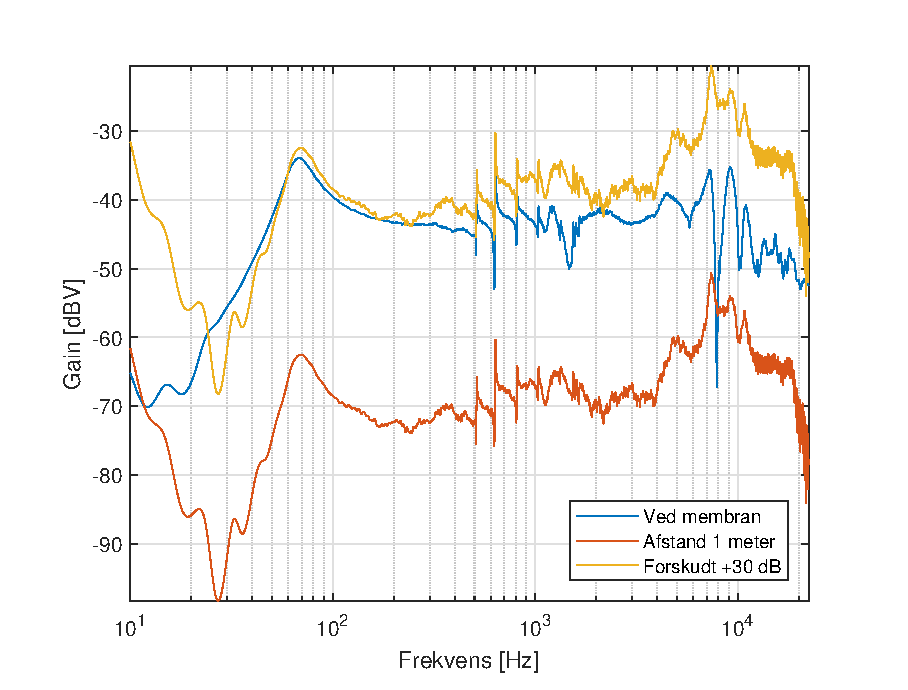
\includegraphics[width=\textwidth]{Pics/ClosedCabinet}
	\caption{Målinger på et lukket kabinet}
\end{figure}\fixme{inkluder simulering i figuren. Derudover ville lidt teori om frekvenskarakteristikken for et lukket kabinet være lækkert, inden vi kaster os ud i målinger. Også så vi kan sammenholde teori med praksis -AB}

Det ses på figuren at, den første resonansfrekvens $f_s$ ligger ved omkring \SI{70}{\hertz} og at forstærkningen stiger med omkring 18 dB/oktav i det fjederstyrede område - altså området under resonansfrekvensen.

Hvis det antages, at det massestyrede område er omtrent en dekade bred i frekvensspektret, så vil dette område derfor ligge mellem \SI{70}{\hertz} og \SI{700}{\hertz}. Herefter vil direktiviteten begynde at spille en rolle for karakteristikkens udseende.\fixme{Det massestyrede område, er vel hele området over fs, er det ikke? Direktiviteten har ikke noget med fjederstyret/massestyret område at gøre, har det? - AB}
 
Det ses også, at når CLIO-mikrofonen flyttes længere væk fra membranen, så bevarer karakteristikken nogenlunde sin form i det massestyrede område og et godt stykke ind i både området over og under i frekvensspektret. Den største forskel er dog, at karakteristikken er blevet forskudt med omkring -30 dB\fixme{Det er vel ikke forskudt. Det er dæmpet/Lavere - AB}. Derfor er den ovenstående kurve målt i 1 meters afstand også blevet korrigeret med +30 dB for at vise dette. \fixme{Vi behøver vel ikke korrigere? Vi skal bare holde 1m afstand-måling sammen med 1m afstand, og tæt afstand med tæt afstand}

For at eftervise at dette er korrekt, så ses der på den nedenstående formel der giver en sammenhæng mellem lydtryk og afstand fra lydgiveren:
\begin{equation}
	L_2 = L_1 - \left| 20 \cdot \log \left( \frac{r_1}{r_2} \right) \right|
\end{equation}

Hvor værdierne $L_1$ og $L_2$ er lydtryksniveauet målt i afstandene $r_1$ og $r_2$. Hvis der ses peaken omkring den første resonansfrekvens $f_s$, så ligger denne ved omkring $-\SI{34}{\decibel}$ når der måles tæt på højtaleren og $-\SI{62.5}{\decibel}$, når der måles i 1 meters afstand. Hvis disse værdier indsættes i den førnævnte formel, så findes der følgende:
\begin{equation}
	\SI{-62.5}{\decibel} = \SI{-34}{\decibel} - \left| 20 \cdot \log \left( \frac{r_1}{\SI{1.00}{\meter}} \right)\right| \quad \Rightarrow \quad r_1 \approxeq \SI{3}{\centi\meter}
\end{equation}

Hvilket altså vil sige, at CLIO-mikrofonen har været placeret omkring \SI{3}{\centi\meter} fra højtaleren. Dette virker også meget sandsynligt.

Grunden til afvigelsen i det fjederstyrede område\fixme{ift hvad? - AB} kan skyldes, at dæmpningsfaktoren i luft er meget anderledes ved lave frekvenser\fixme{ref? - AB}. Afvigelsen ved de højere frekvenser skyldes at direktiviten spiller ind. Det kan derfor sagtens tænkes, at CLIO-mikrofonen ikke har stået præcist vinkelret ind på højtalerens midte. \fixme{Men netop de lavere frekvenser burde vel være ligeglade, da der her ikke spiller direktivitet ind (fjederstyret område) - AB}
\subsection{Indflydelse af basrefleks}
Højtalerkabinettet har et hul på forsiden, på siden og et på bagsiden hvori det er muligt, at installere basreflekser i forskellige længder - dog kun en basrefleks ad gangen. I første omgang er der kun blevet set på hvordan basreflekser af forskellige længder påvirker membranens karakteristik, når basrefleksen er placeret foran på højtaleren. Resultatet af disse målinger i vist på den nedenstående figur:
\begin{figure}[H]
	\centering
	\vspace{-12pt}
	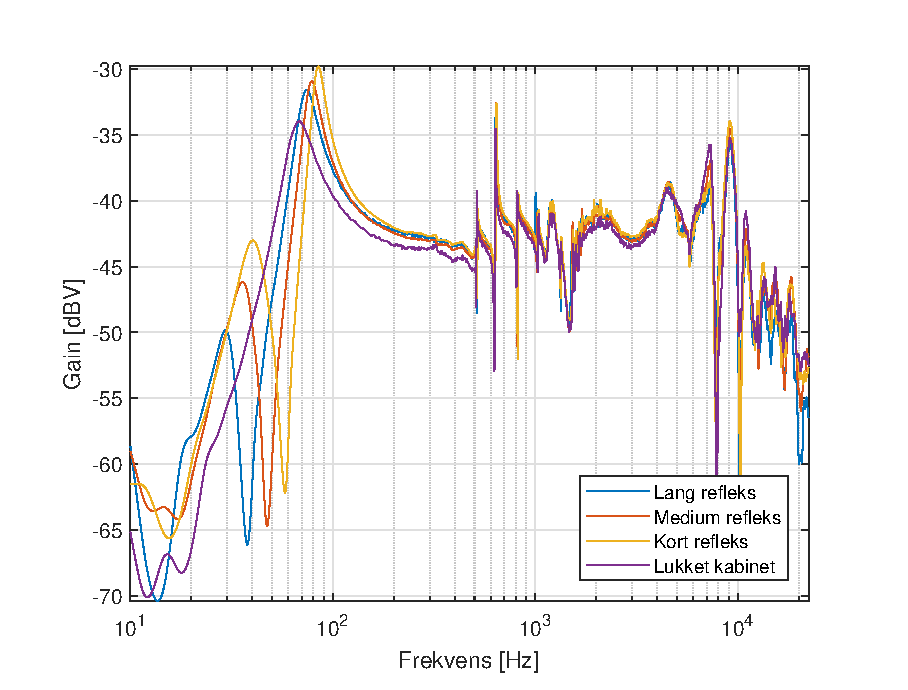
\includegraphics[width=\textwidth]{Pics/BassReflexMembrane}
	\caption{Indflydelse af forskellige længder basrefleks}
\end{figure}

På figuren ses også frekvenskarakteristikken for et lukket kabinet - altså et kabinet uden basrefleks. Det ses, at det lukkede kabinets frekvenskarakteristik er meget lav ved de lave frekvenser. Det ses også, at der tilføjes et forstærkningspeak når der tilføjes en basrefleks. Placeringen af denne peak afhænger af refleksens længde. Jo længere røret er, jo længere nede i frekvensspektret kommer peaken til at ligge. Omvendt vil en længere basrefleks også betyde, at peaken bliver mindre - altså mindre forstærkning.
\begin{table}[H]
	\centering
	\begin{tabular}{l|c|c|c|c}
		& Lukket kabinet & Lang refleks & Medium refleks & Kort refleks \\ \hline
		Dyk fra enhed {[}Hz{]}    & -              & 38              & 47                & 58             \\
		Dyk fra enhed {[}dB{]}    & -              & -66             & -65               & -62            \\
		Peakfrekvens {[}Hz{]}     & 68             & 74              & 78                & 85             \\
		Peakforstærkning {[}dB{]} & -34            & -32             & -31               & -30           
	\end{tabular}
	\caption{Måleresultater}
\end{table}

Ud fra den ovenstående figur ses det også, at basrefleksen ikke vil påvirke membranens frekvenskarakteristik ved frekvenser over \SI{500}{\hertz}.